\documentclass[11pt,a4paper,english]{article}
    \usepackage[latin1]{inputenc}
    \usepackage{amsmath,amsfonts,amssymb}
    \usepackage{enumitem}
    \usepackage{fullpage}
    \usepackage{graphicx}
    \usepackage{tabto}
    \usepackage{etoolbox}
    \usepackage{xcolor}
    \usepackage{hyperref}
    \usepackage{minted}
    \usepackage{parskip}
    \usepackage[title]{appendix}
    \usepackage[font=small,labelfont=bf]{caption}
    \hypersetup{ colorlinks = true}
    \graphicspath{ {./} }

    \title{Bayesian Data Analysis - Assignment 7}
    \author{}

    \begin{document}
        \maketitle
      \definecolor{bg}{rgb}{0.95,0.95,0.95}

        \section{Question}
          Before analyzing the predictions, it will be beneficial to plot the data and look at the trend. We can do that simply by:
          \begin{minted}[bgcolor=bg,fontsize=\small,autogobble]{python}
            plt.plot(years, drowning)
            z = np.polyfit(years, drowning, 1)
            trend = np.poly1d(z)
            plt.plot(years, trend(years), 'r--')
            plt.savefig('./ex7/report/drowining.png')
          \end{minted}

          \begin{center}
            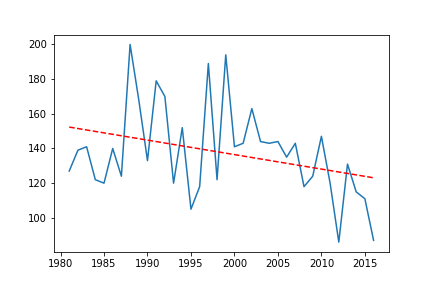
\includegraphics[width=10cm]{drowining.png}
            \captionof{figure}{Number of people drown per year in Finland.}
          \end{center}

          From the trend we can see that the number of drown in Finland is decreasing.

        \subsection{Stan code}
          The $stan$ code described in the question 1 description had 2 main issues:
          \begin{itemize}
            \item
              There was no lower bound for $sigma$. It was declared as $real \ sigma$. This is not good, as it might lead to some miscalculations. The correct declaration is:
              \begin{minted}[bgcolor=bg,fontsize=\small,autogobble]{python}
                real<lower=0> sigma
              \end{minted}
            \item
              The second issue was in \textit{generated quantities}:
              \begin{minted}[bgcolor=bg,fontsize=\small,autogobble]{python}
                ypred=normal_rng(mu, sigma)
              \end{minted}
              That is incorrect because we have to evaluate the prediction on years, which is $xpred$. The correct declaration is:
              \begin{minted}[bgcolor=bg,fontsize=\small,autogobble]{python}
                ypred = normal_rng(alpha + beta * xpred, sigma);
              \end{minted}
          \end{itemize}

        \subsection{Nmerical value of $\tau$}
          \begin{itemize}
            \item The numerical value of $\tau$ is:
              \begin{align*}
                \tau=26.78888...
              \end{align*}
              It was calculate by putting various value into $scale$ and checking the statement $dist.cdf(-69)$:
              \begin{minted}[bgcolor=bg,fontsize=\small,autogobble]{python}
                dist = norm(loc=0, scale=26.78)
                print(dist.cdf(-69))
              \end{minted}
              The value of $dist.cdf(-69)$ should be $0.1/2$ for the correct $\tau$.
          \end{itemize}

        \subsection{Prior in the stan model}
          \begin{itemize}
            \item
              The initial value of both $\alpha$ and $\beta$ in stan model were taken from uniform prior. That was changed for $\beta$ to weekly-informative prior:
              \begin{minted}[bgcolor=bg,fontsize=\small,autogobble]{python}
                beta ~ normal(0, tau);
              \end{minted}
              Please look at \textit{Appendix A  Source code for Question 1} for details.
          \end{itemize}

        \subsection{Predictions for 2019}
          After we have built our stan model, we can predict any upcoming year simply by writing:

          \begin{minted}[bgcolor=bg,fontsize=\small,autogobble]{python}
            data = dict(
              N=len(years),
              x=years,
              y=drowning,
              xpred=2019,
              tau=26.78,
            )
            fit = stan_model.sampling(data=data)
            y_pred = fit.extract()['ypred']
            plt.hist(y_pred, bins=20, ec='white')
          \end{minted}

          And that will give us the predictions as:
          \begin{minted}[bgcolor=bg,fontsize=\small,autogobble]{python}
                    mean se_mean     sd   2.5%    25%    50%    75%  97.5%  n_eff   Rhat
            alpha  1809.3   23.27 827.88 177.23 1269.3 1797.3 2371.9 3436.3   1266    1.0
            beta    -0.84    0.01   0.41  -1.65  -1.12  -0.83  -0.57  -0.02   1266    1.0
            sigma    26.4    0.09   3.24  20.86  24.15  26.11  28.36  33.52   1376    1.0
            mu[1]  152.33    0.22   8.56 135.69 146.53 152.26 158.08 168.97   1544    1.0
            mu[2]   151.5    0.21   8.21 135.56 145.94  151.5 157.07  167.4   1576    1.0
            mu[3]  150.66     0.2   7.86 135.32 145.31 150.66 155.96 165.95   1614    1.0
             ...     ...      ...    ...   ...   ...    ...    ...    ...     ...     ...
            mu[36] 123.06    0.21   8.41 106.21 117.51 123.01 128.62 139.86   1597    1.0
            ypred  121.19    0.54  28.65  64.71 101.84 120.69 140.59 177.37   2824    1.0
          \end{minted}
          As we can see from the above table the the $ypred$ is the prediction for 2019 which is $121$ drowning.
          \begin{center}
            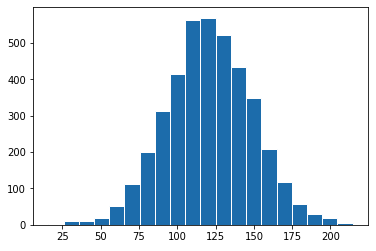
\includegraphics[width=10cm]{drowning_y_prediction.png}
            \captionof{figure}{Histogram of prediction for 2019.}
          \end{center}

      \section{Question}
        \subsection{Pooled model}
          In the pooled model all the machines are considered as one entity, thus we have to combine the all the measurements into one and perform our prediction on the whole data; rather than a subset. With that in mind, we have to first read the data and then flatten it into one array:
          \begin{minted}[bgcolor=bg,fontsize=\small,autogobble]{python}
            machines = pd.read_fwf('./ex7/factory.txt', header=None).values
            machines_pooled = machines.flatten()
          \end{minted}
          The stan model for this is stated in the \textit{Appendix B  Source code for Question 2}.

          \begin{itemize}
            \item \textit{the posterior distribution of the mean of the quality measurements of the sixth machine}: \\
              As we combined all the measurements into one, the $\mu$ value will be the same for sixth machine, seventh machine or all the machines combined. As mentioned before we don't treat each machine as a separate entity, that's exacly the reason why all the $\mu$ will be equal. This is how the histogram looks like:
              \begin{center}
                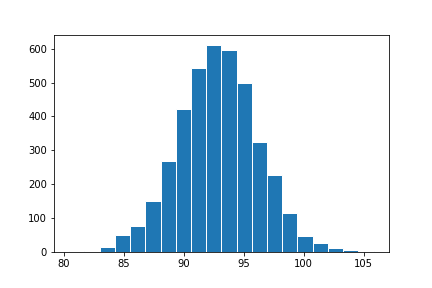
\includegraphics[width=10cm]{pooled_hist_mu.png}
                \captionof{figure}{$\mu$ histogram with pooled model for 6th, 7th or all machines combined.}
              \end{center}

            \item \textit{the predictive distribution for another quality measurement of the sixth machine}: \\
              The prediction will be the same for sixth machine or all combined. We can use the stan to make the predictions:
              \begin{minted}[bgcolor=bg,fontsize=\small,autogobble]{python}
                fit_pooled = model_pooled.sampling(data=data_pooled)
              \end{minted}
              Which gives us this table:
              \begin{minted}[bgcolor=bg,fontsize=\small,autogobble]{python}
                        mean se_mean     sd   2.5%    25%    50%    75%  97.5%  n_eff   Rhat
                mu     92.87    0.06   3.35  86.22  90.65  92.87  95.06  99.41   2748    1.0
                sigma  18.77    0.05   2.55   14.6  16.94   18.5  20.32  24.68   2468    1.0
                ypred  93.33    0.32  19.08  55.19  80.93  93.76 105.58 130.87   3550    1.0
                lp__   -99.3    0.02   0.99 -102.0 -99.66 -99.01  -98.6 -98.35   1759    1.0
              \end{minted}
              The prediction histogram looks like this:
              \begin{center}
                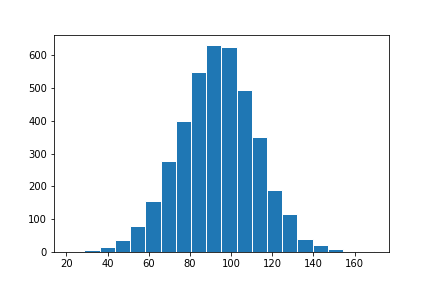
\includegraphics[width=10cm]{pooled_hist.png}
                \captionof{figure}{Prediction histogram with pooled model both for the sixth machine and all combined.}
              \end{center}
            \item \textit{the posterior distribution of the mean of the quality measurements of the seventh machine}: \\
              The answer is stated above in the \textit{the posterior distribution of the mean of the quality measurements of the sixth machine} section.
          \end{itemize}







        \subsection{Separate model}
          In the separate model we treat every machine as an individual entity, thus when calculating $\sigma$ or $\mu$ we take into consideration only a single machine. The combination of all machines should not effect $\sigma$ or $\mu$. The stan model for this is stated in the \textit{Appendix B  Source code for Question 2}

          \begin{itemize}
            \item \textit{the posterior distribution of the mean of the quality measurements of the sixth machine}: \\
              This can be calculated simply by:
              \begin{minted}[bgcolor=bg,fontsize=\small,autogobble]{python}
                fit_separate = model_seperate.sampling(data=data_separate, n_jobs=-1)
                print(fit_separate)
              \end{minted}
              This gives us a nice table where we can allocate the $\mu$ of the sixth machine:
              \begin{minted}[bgcolor=bg,fontsize=\small,autogobble]{python}
                          mean se_mean     sd   2.5%    25%    50%    75%  97.5%  n_eff   Rhat
                mu[1]     75.93    0.36   15.3   44.6  68.25  75.98  83.95 106.05   1833    1.0
                mu[2]    106.57    0.34  10.33  88.75 101.66  106.3 110.89 126.97    944    1.0
                mu[3]      87.8    0.23   9.49  67.93  83.03  87.92  92.65 106.74   1646    1.0
                mu[4]    111.56    0.17   5.91  99.43  108.6 111.52 114.46 123.49   1225    1.0
                mu[5]     89.91    0.27   9.27   70.6  85.84   90.0  94.32 107.29   1143    1.0
                mu[6]     86.45    0.37  14.33  58.26  78.54  86.19   93.8 117.74   1477    1.0
                sigma[1]  30.62    0.55  20.17  13.08  19.47  25.44  34.81  79.54   1352    1.0
                sigma[2]  18.56    0.37  11.89   7.69  11.64  15.26  21.23  52.47   1017    1.0
                sigma[3]  19.64    0.31  12.34   8.41  12.64  16.55  22.55  49.52   1574    1.0
                sigma[4]  12.03     0.2   6.95   4.96    7.6  10.09  14.15  30.48   1265    1.0
                sigma[5]  16.98    0.39   11.8   7.06  10.52  13.68  19.27  46.61    907    1.0
                sigma[6]  30.16     0.5   18.0  12.28  18.87  25.17  35.34  79.14   1289    1.0
                ypred      86.0     0.7  37.13  12.32  67.29  85.77 104.62 162.64   2827    1.0
                lp__     -81.11     0.1   2.99 -88.04 -82.89 -80.75 -78.92 -76.34    913    1.0
              \end{minted}
              Which is \textbf{86.45}. We can also plot the histogram of it:
              \begin{minted}[bgcolor=bg,fontsize=\small,autogobble]{python}
                mu_data_separate = fit_separate.extract()['mu']
                plt.hist(mu_data_separate[:, 5], bins=20, ec='white')
              \end{minted}
              \begin{center}
                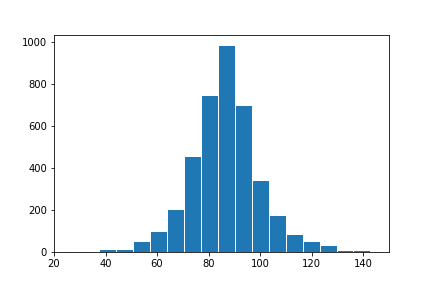
\includegraphics[width=10cm]{separate_hist_mu_six.png}
                \captionof{figure}{$\mu$ histogram with separate model for 6th machine.}
              \end{center}

            \item \textit{the predictive distribution for another quality measurement of the sixth machine}: \\
              The predictive distribution can be extracted from $ypred$.
              \begin{minted}[bgcolor=bg,fontsize=\small,autogobble]{python}
                y_pred_separate = fit_separate.extract()['ypred']
                plt.hist(y_pred_separate, bins=20, ec='white')
              \end{minted}
              \begin{center}
                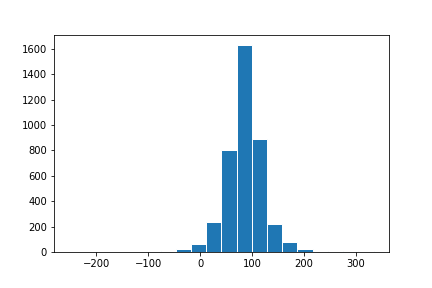
\includegraphics[width=10cm]{separate_hist.png}
                \captionof{figure}{Prediction histogram with separate model for the sixth machine.}
              \end{center}

            \item \textit{the posterior distribution of the mean of the quality measurements of the seventh machine}: \\
              As it was stated before, in the separate model we treat each machine separately. Consequently, we have no any information about the seventh machine. Thus we cannot tell anything about its posterior distribution.
          \end{itemize}

        \subsection{Hierarchical model}
          The hierarchical model is quite interesting. It does treat every machine as a separate entity, but also computes the combination of all the machines as one entity. For that reason it can predict measurements for the machines which have no data. For example, there is no data about the seventh machine, but this model can predict its posterior distribution. The stan model for this is stated in the \textit{Appendix B  Source code for Question 2}.

          \begin{itemize}
            \item \textit{the posterior distribution of the mean of the quality measurements of the sixth machine}: \\
              The same logic, as in separate model, follows here. We start simply by:
              \begin{minted}[bgcolor=bg,fontsize=\small,autogobble]{python}
                fit_hierarchical = model_hierarchical.sampling(data=data_hierarchical, n_jobs=-1)
                print(fit_hierarchical)
              \end{minted}
              Which again, gives us a nice table where we can allocate the $\mu$ of the sixth machine:
              \begin{minted}[bgcolor=bg,fontsize=\small,autogobble]{python}
                        mean se_mean     sd   2.5%    25%    50%    75%  97.5%  n_eff   Rhat
                mu0     92.13    0.36   9.72   71.8  88.13  92.64  97.03 108.53    738    1.0
                sigma0  17.08    0.46  12.29   5.38  10.49  14.32  20.03  45.45    729   1.01
                mu[1]   79.71    0.15   6.56  66.76  75.32  79.65  84.13  92.72   1992    1.0
                mu[2]  103.07    0.14   6.48  90.04  98.92 103.04 107.31 116.52   2247    1.0
                mu[3]   88.89    0.09   6.18  76.41  84.87  88.85  92.92 101.25   4231    1.0
                mu[4]  107.56    0.18   6.68  94.24 103.04 107.69 112.16 120.04   1345    1.0
                mu[5]   90.47     0.1   6.12  78.28  86.59  90.45  94.46 102.45   3904    1.0
                mu[6]   87.32     0.1   6.25  75.07  83.08  87.31  91.64  99.36   3647    1.0
                sigma   15.18    0.06   2.27  11.55  13.55  14.91  16.54  20.41   1572    1.0
                ypred6   87.0    0.26  16.89  52.64  76.11  86.87  98.52  120.0   4076    1.0
                mu7     91.77    0.59  24.43  44.47  82.15   92.6  103.4 133.87   1687    1.0
                lp__   -108.9    0.09   2.52 -114.8 -110.3 -108.4 -107.0 -105.3    755    1.0
              \end{minted}
              Which is \textbf{87.32} and it is quite close to what we had with the separate model: \textbf{86.45}. We can now plot the histogram:
              \begin{minted}[bgcolor=bg,fontsize=\small,autogobble]{python}
                mu_data_hierarchical = fit_hierarchical.extract()['mu']
                plt.hist(mu_data_hierarchical[:, 5], bins=20, ec='white')
              \end{minted}
              \begin{center}
                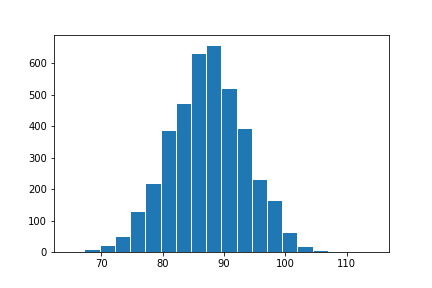
\includegraphics[width=10cm]{hierarchical_hist_mu_six.png}
                \captionof{figure}{$\mu$ histogram with hierarchical model for 6th machine.}
              \end{center}

            \item \textit{the predictive distribution for another quality measurement of the sixth machine}: \\
              The prediction can also be extracted from the above table by:
              \begin{minted}[bgcolor=bg,fontsize=\small,autogobble]{python}
                y_pred_hierarchical = fit_hierarchical.extract()['ypred6']
                plt.hist(y_pred_hierarchical, bins=20, ec='white')
              \end{minted}
              \begin{center}
                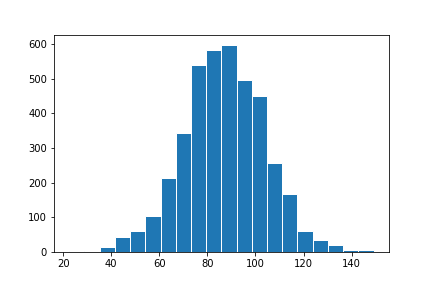
\includegraphics[width=10cm]{hierarchical_hist.png}
                \captionof{figure}{Prediction histogram with hierarchical model for 6th machine.}
              \end{center}

            \item \textit{the posterior distribution of the mean of the quality measurements of the seventh machine}: \\
              Referring to the table we printed above, we can say that the $\mu$ for the seventh machine is \textbf{91.77}. We can now draw the posterior distribution of the mean for the seventh machine simply by:
              \begin{minted}[bgcolor=bg,fontsize=\small,autogobble]{python}
                mu_data_hierarchical_7 = fit_hierarchical.extract()['mu7']
                plt.hist(mu_data_hierarchical_7, bins=20, ec='white')
              \end{minted}
              \begin{center}
                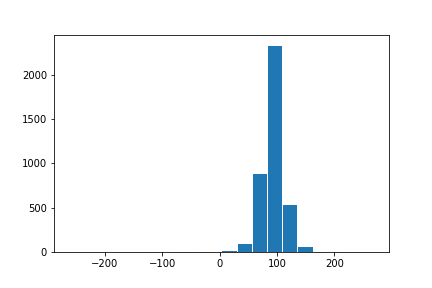
\includegraphics[width=10cm]{hierarchical_hist_mu_7.png}
                \captionof{figure}{$\mu$ histogram with hierarchical model for 7th machine.}
              \end{center}
          \end{itemize}

      \begin{appendices}
        \section{Source code for Question 1}
        \begin{minted}[bgcolor=bg,linenos,fontsize=\small,autogobble]{python}
            import matplotlib
            matplotlib.use('TkAgg')

            from scipy.stats import norm
            import matplotlib.pyplot as plt
            import numpy as np
            import pandas as pd
            import pystan

            drowning_data = pd.read_fwf('./ex7/drowning.txt').values
            years = drowning_data[:, 0]
            drowning = drowning_data[:, 1]


            plt.plot(years, drowning)
            z = np.polyfit(years, drowning, 1)
            trend = np.poly1d(z)
            plt.plot(years, trend(years), 'r--')

            plt.savefig('./ex7/report/drowining.png')
            plt.figure(0)

            stan_code = '''
            data {
            int<lower=0> N; // number of data points
            vector[N] x;    // observation year
            vector[N] y;    // observation number of drowned
            real xpred;     // prediction year
            real tau;
            }
            parameters {
            real alpha;
            real beta;
            real<lower=0> sigma;
            }
            transformed parameters {
            vector[N] mu;
            mu = alpha + beta * x;
            }
            model {
            beta ~ normal(0, tau);
            y ~ normal(mu, sigma);
            }
            generated quantities {
            real ypred;
            ypred = normal_rng(alpha + beta * xpred, sigma);
            }
            '''

            #%% guess of tau
            dist = norm(loc=0, scale=20)
            print(dist.cdf(-69))

            #%% fitting data to stan model
            stan_model = pystan.StanModel(model_code=stan_code)

            data = dict(
                N=len(years),
                x=years,
                y=drowning,
                xpred=2019,
                tau=26.78,
            )

            #%% sampling
            fit = stan_model.sampling(data=data)
            print(fit)

            #%% hist
            y_pred = fit.extract()['ypred']
            plt.hist(y_pred, bins=20, ec='white')
            plt.show()
        \end{minted}

      \section{Source code for Question 2}
        \begin{minted}[bgcolor=bg,linenos,fontsize=\small,autogobble]{python}
          #%%
          import matplotlib
          matplotlib.use('TkAgg')

          from scipy.stats import norm
          import matplotlib.pyplot as plt
          import numpy as np
          import pandas as pd
          import pystan

          #%% The data
          machines = pd.read_fwf('./ex7/factory.txt', header=None).values
          machines_transposed = machines.T

          #%% Pooled model
          '''
          Pooled model
          '''
          stan_code_pooled = '''
          data {
              int<lower=0> N;       // number of data points
              vector[N] y;          //
          }
          parameters {
              real mu;              // group means
              real<lower=0> sigma;  // common std
          }
          model {
              y ~ normal(mu, sigma);
          }
          generated quantities {
              real ypred;
              ypred = normal_rng(mu, sigma);
          }
          '''

          #%% fitting data to stan model
          machines_pooled = machines.flatten()
          model_pooled = pystan.StanModel(model_code=stan_code_pooled)
          data_pooled = dict(
              N=machines_pooled.size,
              y=machines_pooled
          )

          #%% sampling
          fit_pooled = model_pooled.sampling(data=data_pooled)
          print(fit_pooled)

          #%% hist
          y_pred_pooled = fit_pooled.extract()['ypred']
          plt.hist(y_pred_pooled, bins=20, ec='white')
          plt.savefig('./ex7/report/pooled_hist.png')
          plt.figure(0)

          mu = fit_pooled.extract()['mu']
          plt.hist(mu, bins=20, ec='white')
          plt.savefig('./ex7/report/pooled_hist_mu.png')
          plt.figure(0)

          #%% Separate model
          stan_code_separate = '''
          data {
              int<lower=0> N;               // number of data points
              int<lower=0> K;               // number of groups
              int<lower=1,upper=K> x[N];    // group indicator
              vector[N] y;
          }
          parameters {
              vector[K] mu;                 // group means
              vector<lower=0>[K] sigma;     // group stds
          }
          model {
              y ~ normal(mu[x], sigma[x]);
          }
          generated quantities {
              real ypred;
              ypred = normal_rng(mu[6], sigma[6]);
          }
          '''

          #%% fitting data into the stan model
          model_seperate = pystan.StanModel(model_code=stan_code_separate)
          data_separate = dict(
              N=machines_transposed.size,
              K=6,
              x=[
                  1, 1, 1, 1, 1,
                  2, 2, 2, 2, 2,
                  3, 3, 3, 3, 3,
                  4, 4, 4, 4, 4,
                  5, 5, 5, 5, 5,
                  6, 6, 6, 6, 6,
              ],
              y=machines_transposed.flatten()
          )

          #%% sampling
          fit_separate = model_seperate.sampling(data=data_separate, n_jobs=-1)
          print(fit_separate)

          #%% hist
          y_pred_separate = fit_separate.extract()['ypred']
          plt.hist(y_pred_separate, bins=20, ec='white')
          plt.savefig('./ex7/report/separate_hist.png')
          plt.figure(0)

          #%% hist
          mu_data_separate = fit_separate.extract()['mu']
          plt.hist(mu_data_separate[:, 5], bins=20, ec='white')
          plt.savefig('./ex7/report/separate_hist_mu_six.png')
          plt.figure(0)

          #%% Hierarchical model
          stan_code_hierarchical = '''
          data {
              int<lower=0> N;             // number of data points
              int<lower=0> K;             // number of groups
              int<lower=1,upper=K> x[N];  // group indicator
              vector[N] y;
          }
          parameters {
              real mu0;                   // prior mean
              real<lower=0> sigma0;       // prior std
              vector[K] mu;               // group means
              real<lower=0> sigma;        // common std
          }
          model {
              mu ~ normal(mu0, sigma0);
              y ~ normal(mu[x], sigma);
          }
          generated quantities {
              real ypred6;
              real mu7;
              ypred6 = normal_rng(mu[6], sigma);
              mu7 = normal_rng(mu0, sigma0);
          }
          '''

          #%% fitting data into the stan model
          model_hierarchical = pystan.StanModel(model_code=stan_code_hierarchical)
          data_hierarchical = dict(
              N=machines_transposed.size,
              K=6,
              x=[
                  1, 1, 1, 1, 1,
                  2, 2, 2, 2, 2,
                  3, 3, 3, 3, 3,
                  4, 4, 4, 4, 4,
                  5, 5, 5, 5, 5,
                  6, 6, 6, 6, 6,
              ],
              y=machines_transposed.flatten()
          )

          #%% sampling
          fit_hierarchical = model_hierarchical.sampling(data=data_hierarchical, n_jobs=-1)
          print(fit_hierarchical)

          #%% hist
          mu_data_hierarchical = fit_hierarchical.extract()['mu']
          plt.hist(mu_data_hierarchical[:, 5], bins=20, ec='white')
          plt.savefig('./ex7/report/hierarchical_hist_mu_six.png')
          plt.figure(0)

          #%% hist
          y_pred_hierarchical = fit_hierarchical.extract()['ypred6']
          plt.hist(y_pred_hierarchical, bins=20, ec='white')
          plt.savefig('./ex7/report/hierarchical_hist.png')
          plt.figure(0)

          #%% hist
          mu_data_hierarchical_7 = fit_hierarchical.extract()['mu7']
          plt.hist(mu_data_hierarchical_7, bins=20, ec='white')
          plt.savefig('./ex7/report/hierarchical_hist_mu_7.png')
          plt.figure(0)
        \end{minted}
      \end{appendices}
  \end{document}
